\documentclass{siproblemset}

\usepackage{multicol}
\usepackage{xcolor}
\usepackage{mathtools}

% SI Session Information
\course{MTH 1321}
\sessionnum{PT4}
\sessiondate{12/1/21}

% Worksheet Information
\title{Practice Test \#4}
\sections{Chapter 5}
\withnamespace

\definecolor{darkred}{RGB}{110,0,0}

%\debugmode

\begin{document}
    \maketitle
    
    \begin{center}
        \framebox{
            \begin{minipage}{\textwidth}
                \begin{center}
                    \textbf{When completing this practice test, do your best to mimic the test environment:}
                \end{center}
                \begin{enumerate}
                    \item Do not use a calculator.
                    \item Try not to use your notes.
                    \item Time yourself, make sure you are completing the problems at a comfortable pace. Remember that you will only get 55 mins for the actual exam (with fewer questions of course).
                \end{enumerate}
%                \begin{center}
%                    \color{darkred}\textbf{ Please do not share this practice test with anyone else. \underline{Your} commitment to SI and reviewing material earned this, not anyone else's.}
%                \end{center}
%                {\centering When you have finished the practice test, go to the following link to check your answers:\\ \color{blue}{https://baylor.box.com/s/5tjv11enbrssu9xjhrvkesobbz0wx672}\\}
                {\centering \color{blue}When you have finished the practice test, \\check the ``Modules'' section on Canvas for the answer key.\\}
            \end{minipage}
        }
    \end{center}
    
    % Approximating Areas
%    \hspace{-5mm}\textbf{Approximating Areas}
    % UGA-F17-3 6
    \begin{multipartquestion}
        The graph of $y=2^{-x}$ is shown below.
          \begin{center}
            \mbox{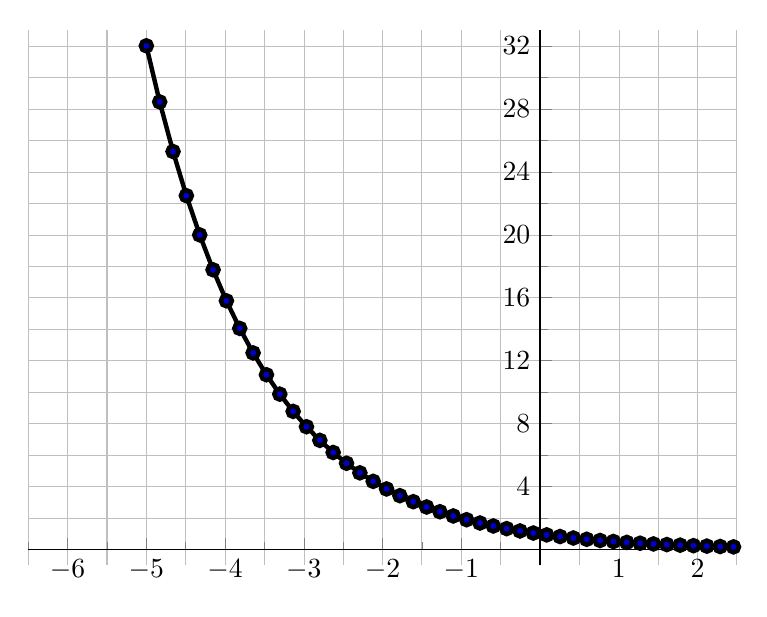
\begin{tikzpicture}[baseline=(current bounding box.north)]
                \begin{axis}[
                x=1cm,
                y=0.20cm,
                ytick distance=4,
                xmin=-6.5,
                xmax=2.5,
                ymin=-1,
                ymax=33,
                grid=both,
                major grid style={line width=.2pt,draw=gray!50},
                minor tick num=1,
                axis x line*=middle,
                axis y line*=middle,
                every axis plot/.append style={ultra thick},
                samples=60
                ]
                \addplot+[black] {2^(-x)};
                \end{axis}
                \end{tikzpicture}}
        \end{center}
        \frq{Estimate the area between the graph of $y=2^{-x}$ and the $x$-axis from $x=-5$ to $x=1$ by finding $L_3$, the left-endpoint approximation with 3 subintervals of equal width. Draw the rectangles you use on the graph above.}
        \Normalsp
        \frq{Considering the rectangles you drew, is the left-endpoint approximation an overestimate or underestimate? What about if we did the right-endpoint approximation instead?}
        \Smallsp
    \end{multipartquestion}
    
    % Definite Integrals
%    \hspace{-5mm}\textbf{Definite Integrals}
    \begin{multipartquestion}
        Use the graph of $f$ below to compute the following definite integrals.
        \begin{center}
            \mbox{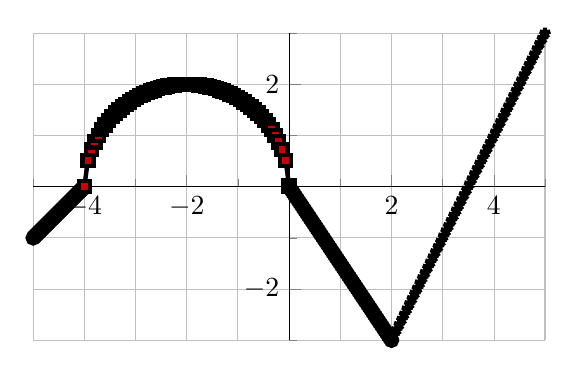
\begin{tikzpicture}[baseline=(current bounding box.north)]
                \begin{axis}[
                x=0.65cm,
                y=0.65cm,
                xmin=-5,
                xmax=5,
                ymin=-3,
                ymax=3,
                grid=both,
                major grid style={line width=.2pt,draw=gray!50},
                minor tick num=1,
                axis x line*=middle,
                axis y line*=middle,
                every axis plot/.append style={ultra thick},
                samples=60
                ]
                \addplot+[black, domain=-5:-4] {x+4};
                \addplot+[black, domain=-4:0] {sqrt(4-(x+2)^2)};
                \addplot+[black, domain=0:2] {-3/2*x};
                \addplot+[black, domain=2:5] {2*x-7};
                \end{axis}
                \end{tikzpicture}}
        \end{center}
        \frq{$\int_{-4}^{2}f(x)\text dx$}
        \tinysp
        \frq{$\int_{5}^{3}f(x)\text dx$}
        \tinysp
        \frq{$\int_{0}^{2}|f(x)|\text dx$}
        \tinysp
        \frq{$\int_{-2}^{2}3f(x)\text dx$}
        \tinysp
    \end{multipartquestion}
\pagebreak
    \mcq{Compute the following definite integrals:}{
        \task $\int_{1}^{e}\left(x+\frac1x\right)\text dx$
        \smallsp
        \task $\int_{3}^{5}e^{-4t}\text dt$
        \smallsp
        \task $\int_{0}^{\pi}\cos(2s)\text ds$
        \smallsp
    }
    
    % Antiderivatives and Indefinite Integrals
%    \hspace{-5mm}\textbf{Antiderivatives and Indefinite Integrals}
    \mcq{Compute the following indefinite integrals:}{
        \task $\int\frac{x^2+5}{2x}\text dx$
        \Smallsp
        \task $\int\paren{2\cos(2x)+e^{4-x}}\text dx$
        \Smallsp
        \task $\int(1+2s+3s^2+4s^3+5s^4)\text ds$
        \Smallsp
        \task $\int(4u)^{3/2}-7u^{1/2}\text du$
        \Smallsp
    }

    % Initial Value
%    \hspace{-5mm}\textbf{Initial Value}
    \frq{Find $y(t)$ when $\dddf[y]{t}=(3t+2)^3$, $y(0)=1$.}
    \newpage
    \frq{Find $f(x)$ when $f''(x)=12x$, $f'(0)=1$, $f(0)=2$.}
    \hugesp
    
    % Miscellaneous
%    \hspace{-5mm}\textbf{Miscellaneous}
    \frq{Beginning at $t=0$ with initial velocity 4 m/s, a particle moves in a straight line with acceleration $a(t)=3t^{1/2}$ \si{\meter/\second^2}. Find the distance traveled after 25 s.}
    \newpage
    
    \begin{multipartquestion}
        You begin to heat a pot of water on the stove. At time $t$ (in minutes), the temperature $T$ (in $^{\circ}$F) of the water is recorded below. For $0 \leq t \leq 8$, $T$ is a differentiable function of $t$.
        \begin{center}
            \begin{tabular}{|l|r|r|r|r|r|}
                \hline
                $t$ (min) & 0 & 1 & 3 & 4 & 8 \\
                \hline
                $T$ ($^{\circ}$F) & 100 & 110 & 140 & 160 & 180\\
                \hline
            \end{tabular}
        \end{center}
        \frq{Find the average rate of change of the temperature of the water over $0\leq t\leq8$. Include units.}
        \Smallsp
        \frq{Was there some time $t_0$ between $t = 0$ and $t = 8$ when the instantaneous rate of change of the temperature of the water was $10$$^{\circ}$F/min? Explain why or why not.}
        \Normalsp
        \frq{Estimate $\int_{0}^{8}T(t)\text dt$ using a method of your choice.}
        \newpage
    \end{multipartquestion}
    \frq{Find the exact value of the area between the curve $f(x)$ and the $x$-axis for $-3\leq x\leq -1$ where $f(x)=\dfrac{1}{16}x^2-\dfrac{x+1}{x}$. }
    \hugesp
    
    % REC 14
    \frq{Find the \textbf{total} area between the $x$-axis and $f(x)=x^2-x$ on $[0,2]$.}
    \pagebreak

    % REC 13
    \mcq{Suppose $\int_1^6f(x)\dd x=8$, $\int_1^2f(x)\dd x=2$, and $\int_1^6g(x)\dd x=-5$. Evaluate each of the following by demonstrating knowledge of properties of integrals.}{
        \task $\int_1^6\paren{f(x)+g(x)}\dd x$
        \smallsp
        \task $\int_1^63g(x)\dd x$
        \smallsp
        \task $\int_6^1f(t)\dd t$
        \smallsp
        \task $\int_2^6f(x)\dd x$
        \smallsp
        \task $\int_1^6\paren{3f(x)-2g(x)}\dd x$
        \smallsp
    }
\pagebreak

    % REC 14
    \mcq{Evaluate the following integrals}{
        \task $\int_{-2}^43x^2-x\dd x$
        \smallsp
        \task $\int_{0}^{\frac\pi2}\paren{1+\sin x}\dd x$
        \smallsp
        \task $\int_{0}^{3}e^{2t}\dd t$
        \smallsp
        \task $\int_{0}^{\frac\pi4}\sec^2\theta\dd\theta$
        \smallsp
        \task $\int_{e}^{e^2}\dfrac1x\dd x$
        \smallsp
    }
\pagebreak
    
    % REC 14
    \mcq{Compute the following derivatives.}{
        \task $\dddx\int_{3}^{x}4t^2+7\dd t$
        \Smallsp
        \task $\dddx\int_{-2}^{x}4t^2+7\dd t$
        \Smallsp
        \task $\dddx\int_{3}^{\sin x}4t^2+7\dd t$
        \Smallsp
        \task $\dddf{s}\int_{3}^{2s^3}\abs{\sqrt{t}-t^2}+3\dd t$
        \Smallsp
    }
\pagebreak

    % REC 14
    \mcq{Evaluate the following integrals.}{
        \task $\int\sin(2s)\dd s$
        \Normalsp
        \task $\int\sin^2(x)\cos(x)\dd x$
        \Normalsp
        \task $\int t(t^2+1)^{1/3}\dd t$
        \Normalsp
        \task $\int\dfrac{\paren{\ln\abs{x}}^3-1}{x}\dd x$
        \Normalsp
        \task $\int(1-\tan x)^{3/2}\sec^2{x}\dd x$
        \Normalsp
        \task $\int\dfrac{\dd x}{x\ln x}$
    }
    
\end{document}